\documentclass[11pt, letterpaper, conference, final, twocolumn]{ieeeconf}
\IEEEoverridecommandlockouts
\overrideIEEEmargins

% packages
\usepackage{amsmath, amsfonts, amssymb, bm, enumerate, url}%, flushend}
\usepackage[boxruled, vlined, linesnumbered]{algorithm2e}
\usepackage[usenames, dvipsnames]{color}
\usepackage[pdftex, xetex]{graphicx}
\usepackage[font={small}]{caption}
\usepackage{float, colortbl, tabularx, multirow, subfig, environ}
\usepackage{pgf, tikz}
\usetikzlibrary{arrows,automata}
\usepackage[normalem]{ulem}

\usepackage[bookmarks=true]{hyperref}
\hypersetup{
colorlinks=true, linkcolor=red, citecolor=blue, filecolor=magenta, urlcolor=blue
%linkcolor=black, citecolor=black, filecolor=black, urlcolor=black
}
\usepackage{url, cite}

% macros
\providecommand{\abs}[1]{\ensuremath \left| #1 \right|}
\providecommand{\norm}[1]{\ensuremath \lVert#1\rVert}
\providecommand{\given}{\, \vert \,}
\providecommand{\cal}[1]{\ensuremath \mathcal{#1}}
\providecommand{\qed}{\hfill \mbox{\raggedright \rule{0.1in}{0.1in} } }

\providecommand{\aeq}[1]{\begin{align} #1 \end{align}}
\providecommand{\aeqs}[1]{\begin{align*} #1 \end{align*}}
\providecommand{\beq}[1]{\begin{equation}#1\end{equation}}
\providecommand{\beqs}[1]{\begin{equation*}#1\end{equation*}}
\providecommand{\trm}[1]{\ensuremath \textrm{#1}}
\providecommand{\enum}[2]{\begin{enumerate}[#1]{#2}\end{enumerate}}
\providecommand{\ilist}[1]{\begin{itemize}{#1}\end{itemize}}
\providecommand{\ag}[1]{\ensuremath \left\langle#1\right\rangle}
\providecommand{\bee}{\begin{enumerate}}
\providecommand{\eee}{\end{enumerate}}
\providecommand{\bm}[1]{\begin{bmatrix}#1\end{bmatrix}}

\usepackage{theorem}
\newtheorem{theorem}{Theorem}
\newtheorem{proposition}[theorem]{Proposition}
\newtheorem{lemma}[theorem]{Lemma}
\newtheorem{corollary}[theorem]{Corollary}
\newtheorem{problem}[theorem]{Problem}
%\theoremstyle{definition}
\newtheorem{definition}[theorem]{Definition}
\newtheorem{example}[theorem]{Example}
\newtheorem{note}[theorem]{Note}
\newtheorem{remark}[theorem]{Remark}
%\theoremstyle{plain}
\newtheorem{assumption}[theorem]{Assumption}

\newcommand{\PP}{\ensuremath \mathbb{P}}
\newcommand{\EE}{\ensuremath \mathbb{E}}

% margins
\setlength{\marginparwidth}{0.6in}
\definecolor{darkgreen}{rgb}{0,0.6,0} \newcommand{\dg}{\color{darkgreen}}
\definecolor{fullred}{rgb}{0.85,.0,.1} \newcommand{\fr}{\color{fullred}}
\definecolor{darkblue}{rgb}{0,0,1.0} \newcommand{\db}{\color{darkblue}}
\definecolor{brown}{rgb}{0.54,.27,0} \newcommand{\br}{\color{brown}}

\newcommand{\pcm}[2]{{\dg #1}\marginpar{\tiny\noindent{\raggedright{\dg[PC]}\br{ #2} \par}}}
\newcommand{\vsm}[2]{{\fr #1}\marginpar{\tiny\noindent{\raggedright{\dg[VS]}\db{ #2} \par}}}
%\renewcommand{\margin}[2]{#1}
\newcommand{\ignore}[1]{}

% save space
%\newcommand{\algsize}{\footnotesize}
%\setlength{\floatsep}{0.05in}
%\setlength{\textfloatsep}{0.1in}
%\setlength{\intextsep}{0.05in}
%\setlength{\belowcaptionskip}{0.01in}
%\setlength{\abovecaptionskip}{0.1in}
%\setlength{\abovedisplayskip}{0.08in}
%\setlength{\belowdisplayskip}{0.08in}

\begin{document}
\title{\bf Twitter-based Mood Evaluation
	\thanks{$^*$Department of Chemical Engineering, MIT.\newline Email: \href{mailto:vishnusr@mit.edu}{vishnusr@mit.edu}}
	\thanks{$^\dag$Laboratory of Information and Decision Systems, MIT.\newline Email: \href{mailto:pratikac@mit.edu}{pratikac@mit.edu}}
	\thanks{Note: Equal contribution from both authors}
}
\author{Vishnu Sresht$^*$ \qquad Pratik Chaudhari$^\dag$}
\maketitle

\begin{abstract}
\small{By providing a convenient, readily-accessible way to reach out to a global audience, twitter has revolutionized the way we broadcast our feelings to the rest of the world. In this paper, we guess the mood of a tweet, i.e., we determinine `how positive people feel' at any given moment through an analysis of their tweets. To this end, we introduce a novel source of already classified text corpora for use as training data. Sites like \href{http://mylifeisg.com}{My Life Is G} and \href{http://fmylife.com}{FML} are a hiherto unutilized source of crowd-curated, well classified training data of text snippets of appropriate length. We study the relative efficacies of several commonly employed classification algorithms, including Support Vector Machines, Principle Component Analysis and Naive Bayes classifiers. We discuss a simple method that is motivated from the fact that both positive and negative tweets are generated from a set of latent topics and introduce a classifier that incorporates this information. Finally, we predict the mood of the nation as the deadline for this project submission draws near using geo-tagged tweets.}
\end{abstract}

\section{Introduction}
\label{sec:intro}
In its recent IPO filing, Twitter disclosed to investors that it made a staggering USD 47.5 million by selling it's data to third-party data analyists \cite{wsj_twitter}. The recent purchase of the tweet data-mining startup Topsy, and the popularity of Coursera's online course on Social Network Analysis  bolsters the claim that analyzing social media is both intellectually exciting and financially lucrative \cite{russell2011mining}. As noted by several authors,\cite{ediger2010massive} social media has become the dominant medium for the convection of thought, opinions, and memes. The implication of these network effects can make or break the case for a new brand - so much so that viral marketing on sites like Twitter has become one of the mainstays in the arsenal of the modern day publicist \cite{richardson2002mining}. Through this project, we attempt to leverage two separate sources of short, user contributed, `status updates` to gauge the geospatial distribution of happiness. The first of these sources is a series of sites where users post anecdotal snippets indicating their current state of mind, and the second is a corpus of geo-coded tweets obtained from the Twitter analytics startup Topsy.



\section{Scraping data}
\label{sec:data}

\subsection{Data crawler}
\label{ssec:crawler}

We used a variety of Python libraries to scrape data from certain websites which contain well classified data tagged with sentiments.
\paragraph{MLIG}
Web 3.0 has given birth to a popular website \href{http://mylifeisg.com}{MLIG} which enables people to post short messages expressing how good their life at that particular moment. These documents are a perfect corpora for our purpose since they are tagged by sentiment. This website also enables other uses to rate the particular comment as ``average'' or ``meh'' (lame). We use this to compute a confidence level of the level of positivity for a document. We used another website called LML to obtain positively tagged documents. \pcm{This website has been taken down since some time and we used an internet archive to scrape data from it.}{fix}
\paragraph{FML, LML}
Similar to MLIG, there is a host of other websites like, \href{fmylife.com}{FML} and  that 
\paragraph{Twitter test data}
We used the API for \href{topsy.com}{Topsy} to obtain 1000 geo-tagged tweets in the country. The policies of Topsy for a free account unfortunately limit us to this number.

\subsection{Scoring and Confidence estimation}
\label{ssec:scoring}

A 'downVote' assigned to a snippet from mylifeisg.com or lmylife.com implies
that (in the opinion of the voter) the author's life is not as 'good' as she
claims. Consequently, we can use a score derived from the numbers of upVotes
and downVotes received by each snippet to represent how positive that snippet
really is. With the snippets from fmylife.com, there is a subtle twist to this
argument. A downVote on this site implies that the voter '... deserve[s] it'.
Snippets that obtain more downVotes than upVotes are typically of the form
where the author confesses to some wrongdoing - such as unprotected sex, or
petty theft. For the sake of simplicity, we will invoke the rather Freudian
argument that such acts of wrongdoing increase the author's happiness (at least
in the short term) and therefore, a snippet from fmylife.com with a negative
score represents a positive sentiment.

The score for each snippet is calculated from the numbers of upvotes and
downvotes received by the snippet (on its source site) using Wilson's interval score
%~\cite{miller_interval}. 
This algorithm calculates the lower bound of one-sided interval within which we
can claim (with a given confidence) that the true value of (positive
votes)/(total votes) lies. One of the key assumptions involved in scoring the snippets this way is that `value' of one vote is the same across the different source sites. 

The output of this step comprises two JSON files `positive.jl' and `negative.jl' that contain pre-processed positive and negative snippets respectively.

\subsection{Tokenization}
\label{ssec:tokenization}

In this section, we discuss methods used to clean a word corpus to enable efficient (and good) feature extraction. A typical document in our data-set looks as follows,
\begin{quote}
\small \emph{Today, I was the only one in an elevator when an attractive girl came in, talking on her phone.  She told her friend, ``I have to go, there's a cute guy on this elevator''.  Before I could even react, she turned to me and said, ``Sorry for lying, I really wanted to get off the phone with her''. FML}
\end{quote}
A typical document in our dataset contains a number of words such as articles, time of the day, and propositions, which are inconsequential to the task of classification. We therefore perform a process called ``tokenization and stemming'' of each document. This consists of the following steps:
\enum{1.}{
\item Break the document into individual sentences.
\item Keep only words which do not include any digits and are more than three letters long.
\item Filter out using a stop word dictionary which consists of common articles, propositions, etc.
\item Tag each word using its appropriate part of speed in the sentence. An HMM-based model is used to estimate the correct part of speech for every word. We only use nouns, adjectives and verbs in our analysis.
\item Lemmatize the resulting words: this process converts words such as ``studying'' to ``study'', ``boyfriend's'' to ``boyfriend'' etc. This is an essential step to ensure a good vocabulary construction.
}

A Python based natural language processing library, \href{http://www.nltk.org}{NLTK} was used for steps $3,4,5$ mentioned above. It uses words from \href{http://wordnet.princeton.edu}{Wordnet} to lemmatize and tokenize words in a corpus. The final result of running this sequence of steps on the document described above is the following set of words which quite succinctly captures the incident in the elevator!
\begin{quote}
\emph{attractive, come, cute, elevator, friend, girl, guy, lying, phone, say, tell, today, want}
\end{quote}

\subsection{Discussion}
\label{ssec:discussion}

The word clouds shown in Fig.~\ref{fig:pos_cloud} and Fig.~\ref{fig:neg_cloud} show the highest frequency words in data with positive and negative sentiments respectively. As a comical digression, let us talk briefly about the nature of words in these two sets. It is not surprising that words related to friends such as \emph{guy, friend} are overwhelmingly positive while most negative sentiments are characterized by people complaning about their significant others, e.g., \emph{boyfriend, girlfriend}. Surprisingly, \emph{sex} is often used in a negative connotation while \emph{school, work} are used to express positive sentiments. To conclude, it is fairly obvious that \emph{mom, dad} figure in the second picture.

On a more serious note, a lot of words overlap in the two sets, i.e., a naive algorithm that uses a word dictionary to guess the sentiment is expected to perform very poorly. This will explain the poor performance of Decision Trees in Sec.~\ref{sec:results}.

\begin{figure}[!htp]
\centering
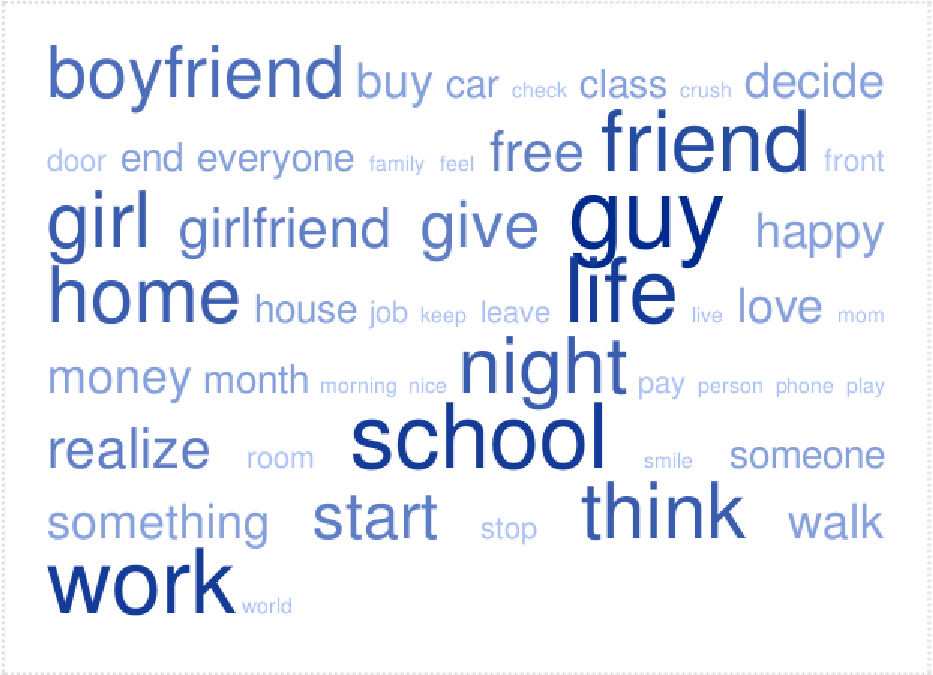
\includegraphics[width= 0.8 \columnwidth]{fig/pos_cloud}
\caption{Word cloud for documents with positive sentiment}
\label{fig:pos_cloud}
\end{figure}
%
\begin{figure}[!htp]
\centering
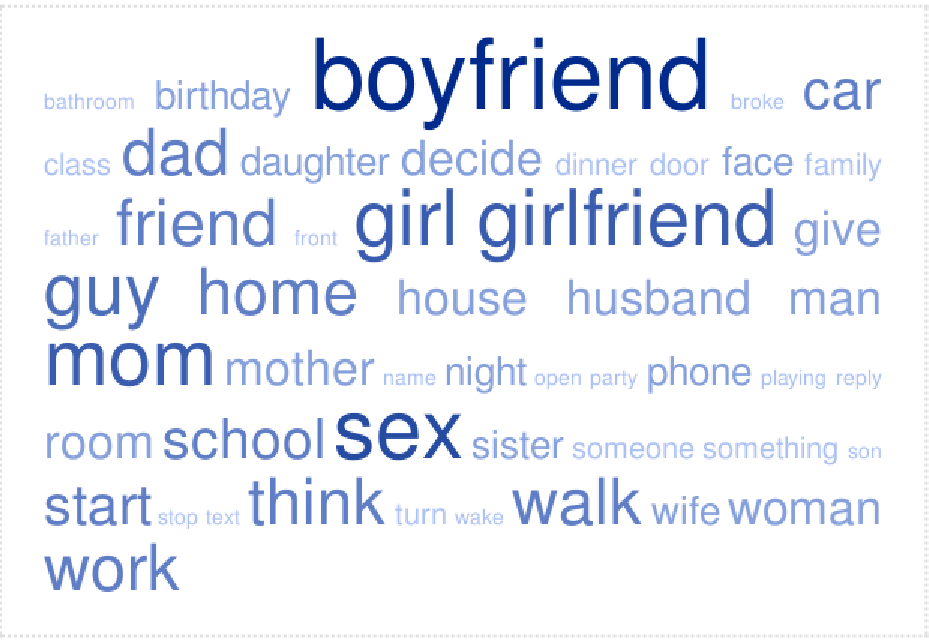
\includegraphics[width= 0.8 \columnwidth]{fig/neg_cloud}
\caption{Word cloud for documents with negative sentiment}
\label{fig:neg_cloud}
\end{figure}

\section{Feature representation}
\label{sec:features}

From the preceeding section, we obtain a set of short documents, let us cay them $D = \{d_1, d_2, \ldots, d_m\}$, with each document $i$ containing a possibly different set of words $w_{i} = \{w_{i,1}, w_{i, 2}, \ldots, w_{i, n_i} \}$. The purpose of this section is to select a good vocabulary of $n$ words, call it $W^*$, from the combined set of words, $W = \{w_1, \ldots, w_m\}$. Given such a set, we obtain a feature vector of length $n$ for every document $d_i$, say $x_i$.
$$
x_i[j] = \begin{cases}
	1 & \trm{ if } w_{i,j} \in W \\
	0 & \trm{ otherwise }
\end{cases}
$$
This results in a set of $n$-dimensional feature vectors $X = \{ x_1, x_2, \ldots, x_m \}$ with labels $Y = \{y_1, y_2, \ldots, y_m \}$. For some algorithms, we map the labels to binary classes, $C = \{c_1, c_2, \ldots, c_m \}$.
$$
c_i = \begin{cases}
	+ & \trm{ if } y_i > 0 \\
	- & \trm{ otherwise }
\end{cases}
$$

We employ four different feature representations:
\paragraph{Word Frequency}
\label{ssec:wf}
We can construct a word frequency map for every word $w \in W$ as,
$$
tf(w) = \sum_{i=1}^m [[ w \in w_i ]]
$$
The vocabulary $W^*$, is then set of words with $n$ highest frequencies.

\paragraph{Information Gain}
\label{ssec:ig}
Information gain is a criterion that quantifies the quality of a feature, i.e., it measures the information required for class prediction of a document based on the persence or absence of a feature. It can be calculated by the decrease in entropy of the data if the feature is included. The information of a set of documents, $D$ is simply,
$$
H(D) = -p_+ \log p_+ - p_- \log p_-
$$
where $p_+ = \PP(+ | d), p_- = \PP(- | d)$ for some arbitary document $d$. In our work, we compute this as $p_+ = \abs{D_+}/\abs{D}$ and similarly for $p_-$, where $D_+$ is the set of all documents tagged as $+$. For $n$-dimensional feature set $X$, we compute
$$
H(D_+ | w) = -\sum_{i=1}^n p_+(w) H(+ | w)
$$
To compute $H(+|w)$, we use $\PP(+ | w) = \PP(+, w)/ \PP(w)$ and 
$$\PP(+, w) = \abs{\{ d: d \in D_+, w \in w_d \}}/\abs{D},$$ 
$$\PP(w) = \abs{\{ d: d \in D, w \in w_d \}}/\abs{D}.$$
Finally,
$$
IG(w) = H(D) - H(D_+ | w) - H(D_{-} | w).
$$

\paragraph{Gain Ratio}
\label{ssec:gr}

The Gain Ratio is an enhanced version of the Information Gain. It normalizes IG by the entropy of the word itself, i.e.,
$$
GR(w) = \frac{IG(w)}{H(w)}
$$
where $H(w)$ is computed using $p_w$ as described in the previous paragraph.

\paragraph{TF-IDF}
\label{ssec:tfidf}
We also used an approach inspired by a popular method of constructing small vocabularies from a word corpus called ``term frequency-inverse document frequency''. The first term, i.e., term frequency is already computed in Sec.~\ref{ssec:wf}. Inverse document frequency is defined for a word $w \in W$ as
$$
idf(w) = \log \left[ \frac{\abs{D}}{\abs{\{d: w \in w_d \}}} \right].
$$
The denominator here is the number of documents that a word $w$ appears in. Thus $idf$ penalises words which occur very frequently in documents. The vocabulary $W^*$ is constructed using the words with the highest value of the product $tf(w) * idf(w)$. In conventional TF-IDF formulations, each document has a large number of repeated words, e.g, research papers, which is not true in our case.

We note that this approach gives the best performance for a number of algorithms tested in this report.

\section{Results}
\label{sec:results}

This section uses the feature representation created in Sec.~\ref{sec:features} and shows an analysis of various algorithms and features on the data.
For the algorithms discussed in this section, we used a popular Python library for machine learning called $\tt scikit\_learn$~\cite{scikit-learn}. This library has very efficient and well documented implementations of algorithms which makes it possible to evaluate the performance with different values of parameters. We analyse the data using four different algorithms as described below. Note that the parameters of these algorithms were tuned manually using $3$-fold cross-validation and we report the results using the best parameters for the various feature representations.

\subsection{Support Vector Machine (SVM)}
\label{ssec:svm}

We use the standard SVM introduced in the class with regularization. The regularization parameter $C$ was chosen using cross-validation. Note that using a large value of $C$ is beneficial because the feature vectors are sparse binary strings, i.e., almost all of them are away from the origin. 

\subsection{Principle Component Analysis (PCA)}
\label{ssec:pca}

We were keen on using PCA because the feature vectors in our dataset are extremely sparse. We would like to understand what dimensions of data are particularly useful for a discriminative classifier and keep only those. This should reduce the performance of a discriminative classifier, say SVM slightly, but the tradeoff of computational complexity versus accuracy heavily favors dimensionality reduction in such problems.

PCA works by computing a singular value decomposition of the dataset and keeps only the eigenvectors that are (i) larger than a certain threshold or, (ii) the top few eigenvectors. A few notes about our approach:
\enum{1}{
\item It is often problematic to decide the size of for the reduced sub-space. In our implementation, we compute the percentage variance in the dataset that can be attributed to each dimension of dataset and use it to select the number of components in PCA. As a result, we project the $200$-dimensional feature vector down to about 50 components.
\item We use the implementation of PCA provided by $\tt scikit-learn$. We also process the data to remove the mean of the dataset from every data point. This enables the SVD to converge well in practice.
}


\subsection{Adaboost}
\label{ssec:adaboost}
%
Adaboost is a popular algorithm introduced by Freud and Schapire in~\cite{freund1999short}. The idea here is to fit a sequence of weak learners, e.g., one dimensional decision trees on slightly modified versions of the same data set. The predictions from all these weak learners (along with weights) are collected together to obtain the final classifier. The mathematical formulation and the algorithm is the same as what discussed in the class, in particular this algorithm uses an exponential loss function and uses it as an upper bound for the prediction error.

In our work, we used Decision Trees with a depth of 1, i.e., one dimensional Decision Trees as weak learners in Adaboost. The number of weak learners was set to be 25 after checking a few different values to provide a good tradeoff between training time and prediction accuracy.

\subsection{Naive Bayes classifer (NB)}
\label{ssec:naive_bayes}
%
We are interested in calculating the probability of a label $+$ given all the words in a document, i.e., $\PP(+ \given w_1, \ldots, w_n)$. This can be written as,
\aeqs{
\PP(+ \given w_1, \ldots, w_n) &= \frac{\PP(+)\ \PP(w_1, \ldots, w_n \given + )}{\PP(w_1, \ldots, w_n)}\\
&\propto \PP(+, w_1, \ldots, w_n).
}
The numerator is a product of the prior probability of a class $+$ and the likelihood of generating $w_1, \ldots, w_n$ given $+$ to obtain the posterior on the left hand side. The Naive Bayes classifer works on the simple premise that the joint probability can be factorized as
$$
\PP(+, w_1, \ldots, w_n) = \PP(+) \prod_{i=1}^n \PP(w_i \given +)
$$
i.e., the probabiltiy of generating a class $+$ from individual words $w_i$ is independent of some other word $w_j$. A classifier can be obtained easily from this argument as
$$
h(w_1, \ldots, w_n) = \arg \max_{c \in \{ +, - \} }\ \PP(c) \prod_{i=1}^n \PP(w_i \given c)
$$
%
In other words, it considers unigrams as independent to be each other. Strictly speaking, this is not correct. As Fig.~\ref{fig:pos_cloud} and Fig.~\ref{fig:neg_cloud} show, there are quite a few common words in both data sets and a word like \emph{boyfriend} only shows a markedly different frequency in the two classes. However, for large amounts of data, this effect is less pronounced and we still obtain good classification.

\subsection{Discussion}
\label{ssec:discussion}

Table~\ref{tab:feature_alg} shows the mean of $3$-fold cross-validation scores for various feature representations and different classifiers. A few remarks about these numbers are in order:

\begin{itemize}
\item We have used a weighted version of SVM in our implementation, i.e, each data point is weighted by the confidence estimate
\item Estimates for PCA are very close to those of SVM in spite of having a large reduction in the dimensionality. The number of dimensions in PCA is just 50 as compared to 200 in SVM.
\item Gain Ratio seems to perform better than other approaches such as WF and TF-IDF. This is consistent with the numbers reported in literature.
\end{itemize}

We note that the success ratio in every case is very large. It is surprising that this shows a marked dissimilarity to numbers reported in literature. In most papers, approaches that involve a combination of SVM and TFIDF show a success ratio of 0.82. In fact, this is precisely the kind of numbers that we get if we include only data from FML, LML and MLIG. If we include the data from the Twitter dataset, which is tagged manually, we get much higher prediction success. This can be attributed to the fact that upvotes and downvotes on these websites incorporate elements such as sarcasm, mockery etc. The scoring and confidence estimates that we compute from these are skewed do to this.

\begin{figure}[H]
\centering
\vspace{0.1in}
\begin{tabular}{ |c|c|c|c|c| }
  \hline
  Feature & SVM & PCA & Adaboost & NB \\[0.03in]
  \hline
  WF & 0.935 & 0.926 & 0.936 & 0.936\\
  IG & 0.938 & 0.930 & 0.936 & 0.939\\
  GR & 0.942 & 0.944 & 0.933 & 0.938\\
  TF-IDF & 0.926 & 0.926 & 0.936 & 0.936\\
  \hline
\end{tabular}
\caption{3-fold cross validation success ratio estimates for different feature representations and algorithms}
\label{tab:feature_alg}
\end{figure}


\section{Latent topics}
\label{sec:latent}

The previous section demonstrated the performance of various classifers on the feature representations obtained from the data. This section builds upon the idea that words in a document are results of a few latent topics. In other words, rather than training a classifer to distinguish between words, we train it to distinguish between latent topics. The analysis in this section is inspired by~\cite{nikolov2012nonparametric}.

This idea has been pursued in literature in a number of different ways. Let us note a popular line of research that introduces supervised learning for topic models~\cite{blei2010supervised}. The idea here is to classify using 

Suppose that for the two classes, $+$ (documents that express positive sentiment) and $-$ (documents that express a negative sentiment), we have a set of latent topics. Let $p = \{ p_1, \ldots, p_m \}$ be the topics that result in words associated with $+$ and $q = \{ q_1, \ldots, q_n \}$ be the topics that result in words associated with $-$. Each sentiment $+$, $-$ is a noisy observation based upon these latent topics. However, we do not know what these topics are and hence we create a simple model for them.

Denote the words in a document by $s$. Let the probability of generating an observation $s$ from latent topics $p$ be,
$$
\PP(s\ \trm{generated from}\ p) \propto e^{-\gamma\ d(s, p)}
$$
where $d(s,p)$ is some positive definite function that metric and $\gamma$ is a tunable parameter. Note that we need $d(s,p)$ to be symmetric. In our work, we use the Hamming distance between two feature representations as the function $d(\cdot, \cdot)$. We make use of the set of observations, i.e., words in documents to classify a new document. Let $R_+$ be the set of all reference documents that are maked as $+$, $R_-$ is defined similarly. The probability of a new signal $s$ belonging to $+$ is then,

\aeqs{
\PP(+ \given s) &= \sum_{r \in R_+}\ \PP(s\ \trm{in}\ +, s\ \trm{shares a latent source with } r)\\
&= \sum_{r \in R_+} \sum_{j=1}^n \PP(s \trm{ generated by } p_j, r \trm{ generated by } p_j)\\
&\propto  \sum_{r \in R_+} \sum_{j=1}^n \exp(-\gamma[ d(s, p_j) + d(r, p_j)])\\
&\sim \sum_{r \in R_+} \exp \left( -\gamma \min_j [ d(s, p_j) + d(r, p_j)] \right)
}
Finally,
\beq{
\PP(+ \given s) \sim \sum_{r \in R_+} \exp \left(-C\ \gamma d(s,r) \right)
\label{eq:latent_topic}
}
The second last approximation is obtained as follows: We see that for a large $\gamma$, the summation $\sum_{j=1}^n$ is dominated by the term with the minimum exponent. On the other hand, the last approximation is obtained by noting that the minimum over all terms of the form $[ d(s, p_j) + d(r, p_j)]$ over all signals in $p$ is of the form $C d(s,r)$ for some $C > 0$ and is achieved at $p^* = (s+r)/2$. It is easy to see that this is a valid approximation when the latent source $p_{j^*}$ is close to the global minimizer $p^*$. We can approximate $\PP(- \given s)$ similarly. 
%We can however, also use the weights of each document that were obtained in Sec.~\ref{ssec:scoring} to get a weighted average of elements in $R_+$ as
%$$
%\PP(+ \given s) \sim \sum_{r \in R_+} y_r \exp \left(-C\ \gamma d(s,r) \right).
%$$

\begin{figure}
\centering
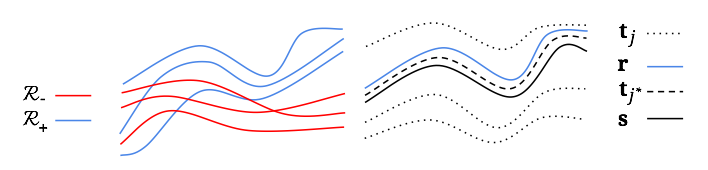
\includegraphics[width=\columnwidth]{fig/latent_topics}
\caption{This figure shows the various classes of positive and negative sentiments and motivates the approximation made in Eqn.~\eqref{eq:latent_topic}.}
\label{fig:latent_topics}
\end{figure}

The crux of this approach is that we cannot compare observations, i.e., words in documents to latent signals because we do not know them. Instead, we compare words to reference words in the traning data itself and obtain a simple rule for a discriminative classifier. Let $R(s) = \PP(+ \given s)/\PP(- \given s)$ and $\theta$ be a threshold. We classify the observation according to the function $f(s) = \trm{sign}(R(s) - \theta)$. It is clear that $\theta > 1$, set its value to $1.25$ because we would like make fewer mistakes while classifying a tweet as $+$, a funny example of where this was not done would be~\cite{target_pregnant}.

\paragraph{Results}
We bootstraped the data to perform cross-validation and computed the prediction error on a randomly sampled subset of the data. The size of the bootstrapped data is 0.7 times the original dataset and the size of the test data is 0.2 times that of the original dataset. We did this because computing the discriminative classifier is prohibitive for a large dataset. We obtain a success ratio of 0.874 for classifying positive samples and 0.96 for classifying negative samples. This is consistent with the fact that we set $\theta = 1.25$, we are more conservative while classifying a sentiment as positive.


\begin{figure*}
\centering
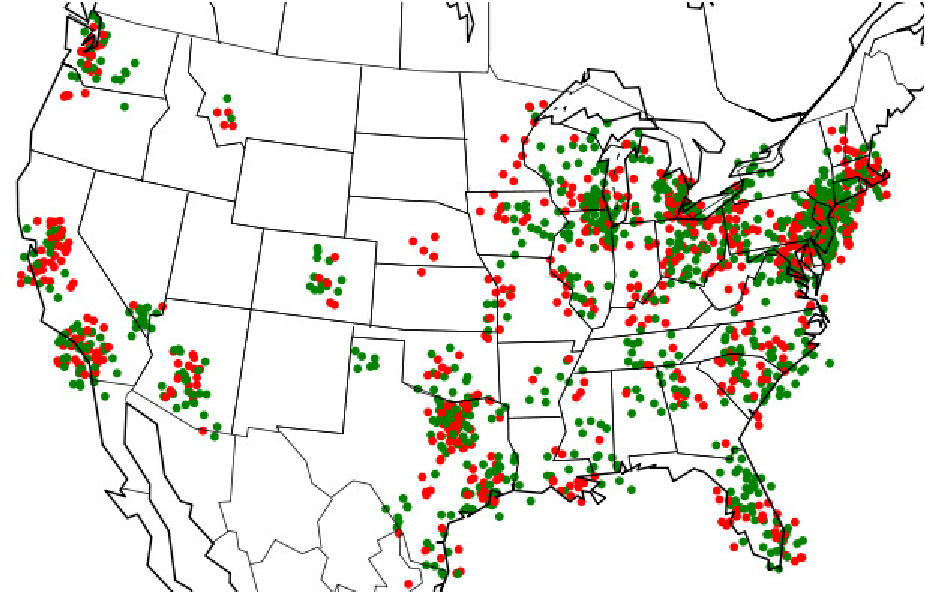
\includegraphics[width=1.5 \columnwidth]{fig/map.pdf}
\caption{Mood map of USA}
\label{fig:map}
\end{figure*}

\section{Test Data}
\label{sec:test_data}

Fig.~\ref{fig:map} shows the mood map of USA at about midnight of Thursday, Dec. 5$^{th}$. Note that the frequency of data points correlates highly with the population density of various areas. Also, some cities are clearly more twitter savvy than others as is evidenced by the complete lack of data points in the mid-west. 
\enum{1.}{
\item Some cities are also clearly more happy than others. In particular, note that Chicago on the west coast of Lake Superior is extremely happy while Detroit, a little right to it, on the boundary of Lake Michigan is not that happy. The east coast, in particular, New York has a lot of green data points, while Boston seems to be particularly unhappy, keeping with the angry-Bostoners stereotype.
%
\item Southern California with a much warmer weather is noticably happier than San Francisco.
}

\section{Conclusions}
This paper used novel data corpora from websites such as FML and MLIG that are already tagged according to the sentiment by users. We employ a number of feature representations on this dataset 

we guess the mood of a tweet, i.e., we determinine `how positive people feel' at any given moment through an analysis of their tweets. To this end, we introduce a novel source of already classified text corpora for use as training data. Sites like \href{http://mylifeisg.com}{My Life Is G} and \href{http://fmylife.com}{FML} are a hiherto unutilized source of crowd-curated, well classified training data of text snippets of appropriate length. 
We study the relative efficacies of several commonly employed classification algorithms, including Support Vector Machines, Principle Component Analysis and Naive Bayes classifiers. We discuss a simple method that is motivated from the fact that both positive and negative tweets are generated from a set of latent topics and introduce a classifier that incorporates this information. Finally, we predict the mood of the nation as the deadline for this project submission draws near using geo-tagged tweets.

\bibliography{writeup}
\bibliographystyle{unsrt}

\end{document}

